\section{Introduction}
% Just a first sketch:
This Bachelor Thesis is about writing a fast and interactive 3D visualization environment for scientific computing. 
The focus is on usability, applied to all the different interfaces, ranging from abstract API interfaces to graphical user interfaces. 
The ultimate goal is to make scientific computing more accessible to the user.
As \ac{GUI} elements and editable text fields are supplied, one can also write and execute scripts.
Using these widgets, all bound variables can be visualized and some of them can be edited interactively. 
This can be used as a basis for interactive programming or visual debugging, further helping the user to understand his algorithms.

The introduction is structured in the following way.
First, an introduction to the general field of research and its challenges is given. 
From these challenges, the problems relevant to this thesis will be extracted.
Finally this chapter will conclude with a solution to the problem, how to measure the success and give an outlook on the structure of the entire Bachelor Thesis.


\subsection{Scientific Computing}
Scientific computing is the area of computing that evolves around all kind of scientific research.
It is a very broad field involving a lot of different challenges. 
In some areas like particle physics, the problems are computationally so demanding, that they can only be solved with the help of super computers.
In other areas like robotics, it is important to be efficient, because the algorithms are running on embedded systems with limited resources. 
In a lot of other areas, speed does not need to be important, but it can be that the algorithm in itself is very difficult to comprehend. 
So the more comprehendable an algorithm can be written down in a programming language, the easier it will be to actually implement the algorithm without errors.
Above all, programming itself is secondary to the research goal.
This means, that it can be expected that a researcher just has rudimentary programming skills and that he wants to put as little time as possible into solving programming problems.
So things like manual memory management and difficult design patterns with a lot of boilerplates are to be avoided in scientific computing.
This has lead to the rise of programming languages and tools specifically tailored to scientific computing.
The most prominent examples include Mathematica, R and Matlab.
They all aim to provide simple syntax for linear algebra and statistical code, while taking away programmatically difficult tasks like memory management. Also, they come with a rich standard library, which means most research can be done without loading any additional module, which makes them great tools for rapid prototyping.
At the current state, the speed of these languages suffer from the high level of abstraction. In order to cater to the fields of scientific computing which is in need of highly performant code, a lot of the core is written in another language like C/C++ and Fortran. This poses a problem in itself. 
As soon as a researcher needs to do something out of the ordinary in a performant way, he needs to switch to a fast multi purpose language. So in the end he is loosing all the advantages of the high level scientific computing language.
A pattern which has evolved out of this dilemma is to prototype in a nice high level language and as soon as the algorithms has been confirmed to work, to rewrite it in a fast low level language.
One of the first language promising to solve this dilemma for scientific computing is Julia. 
It is supposed to be high level and optimized for the work of scientific computing while approaching the speed of statically compiled languages like C.
This leads us straight to the contribution of this thesis.

\subsection{Contribution}

The goal is to bring the speed and usability of Julia to a scientific visualization library.
On top of that, the library should make it simple to interact with complex algorithms and form a basis for visual debugging these.
The interaction part means, that it must be possible to change values over time.
Visualizing data that changes over time is very sensitive to latency. 
If you can not calculate every value in time for a single frame, you either need to skip frames or delay them.
This leads to stutters, which, depending on the magnitude, can be unpleasant or completely corrupt the work-flow.
Which makes it important, that every routine that is used in the visualization pipeline is as fast as possible.
This is only possible, if everything is written in a fast language with as little conversations and memory transfers as possible. If the link between two languages can not be guaranteed to be fast, from this also follows, that everything should be written in one language.
This has been achieved by writing Romeo in Julia and is the main contribution in this thesis.
As the chosen language is also a high-level language and some effort was put into creating a concise architecture, a further contribution is, that the development cycles can be very short and the library is easy to extend.
Another contribution is the interactivity of the visualizations via simple widgets, which allow you to change the appearance of large datasets or the datasets themselves without any stutters.
With these elements, it has also been achieved to build a basis for simple visual debugging.


\subsection{Field of Research and Problem}

\vspace{1em}
\begin{minipage}{\linewidth}
    \centering
    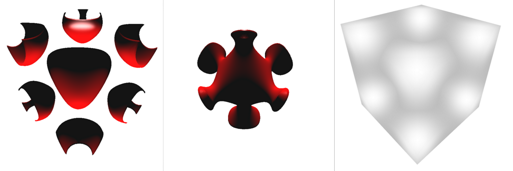
\includegraphics[width=0.7\linewidth]{graphics/surfaces.png}
    \captionof{figure}[Volume Visualization]{different visualizations of $f(x,y,z)=\sin(\frac{x}{15})+\sin(\frac{y}{15})+\sin(\frac{z}{15})$, visualized with Romeo. From left to right: Isosurface with isovalue=0.76, Isosurface with isovalue=0.37, maximum value projection}
    \label{fig:volume}
\end{minipage}
\vspace{1em}

%Scientific computing: visual debugging, interactive programming, high performance
%First rough sketch:

This thesis is about bringing performance and usability together in the realms of scientific computing and 3D visualizations.
These two demands are pretty much opposing concepts. One is about bringing tasks into a form of making them best understandable to humans, and the other is about transforming a task to make it fit well to a computer architecture.
These two tasks could not be more different. For humans, data and algorithms becomes understandable if they are high level and represented visualy, auditorial or tactile together with immidiate feedback. 
It is the task of making problems accessible to a human, who has evolved his capabilities in order to survive and find food and not to create complex algorithms.
Computers on the other hand love to have their registers filled optimally, move memory to smaller and faster caches and dislike random access to memory. That is all they care about, whether a human understands this or not.

To close this gaps, compiler have been created. They are translators between human understandable languages to machine instructions.
This is just the first step and many more are needed to create an enjoyable user experience.
These steps range from introducing graphical user interfaces, novel input devices like the mouse, understandable visualizations and so forth.
All these advances have made computers usable even for people who do not have an education in computer science.
In this thesis the field is scientific computing, which still has quite a lot of barriers for novel users.
Scientific computing is usually about implementing mathematical equations, complex algorithms and manipulating and analyzing data.
Most research is done in some specialized, high-level scientific computing language.
Besides the previously discussed performance problems with this approach, the lack of easily usable and fast visualization libraries also poses a problem.
Most state of the art visualization libraries use C++ at their performance critical core, they are not extendable or they are simple toy libraries, which can not be used for projects with higher performance demands.

This is a problem for several reasons.
First, it creates a complexity and performance bottlenecks when interfacing with other languages. The next problem occurs, when the library does not offer the needed functionality and the programmer has to step in and extend the library.
Finally, you often do not have easily accessable GUI elements, they come from a different package (possibly written in yet another language) or they are compliacted to use. 
This makes it hard for the researcher to visualize and interact with his data. It would be desirable, if interactability, speed and extendability would be the default for any visualization library.

Consider the following function $f(x,y,z)=\sin(\frac{x}{15})+\sin(\frac{y}{15})+\sin(\frac{z}{15})$, which describes a 3D volume mathematically. 
This is a simple function, which is already not that easy to interpret. In figure \ref{fig:volume}, you can see different visualizations of f.
If you can interact with this visualization, by moving through the iso values or coloring certain areas, it will make the function more understandable.
This deeper understanding is crucial for identifying problems in the underlying math, extending the function, or explaining it to other people.

In summary, the software in this thesis focuses on research which involves writing short scripts, while playing around with some parameters and visualizing the results.
An example would be a material researcher, who is investigating different 3D shapes and materials and their reaction to pressure.
The researcher would need to read in the 3D object he wants to analyze, have an easy way to tweak the material parameters and it would be preferable to get instant feedback on how the pressure waves propagate through the object.
There are quite a few libraries out there offering this, but none of them is written in a high level language, offers speed, extendability and usability, while being deeply integrated into a scientific programming language.

\subsection{Outlook}
%Structure of BA and a few worts on the results 
[short outlook, includes BA structure and some words about the results]